\section{Materials and Methods}
\label{p1:sec:methods}

\subsection{Subjects}

Seven subjects (6 male, 1 female) provided written informed consent to participate in the experiments. Ages ranged from 23 to 65 years. Subjects were free of any known vestibular or other neurological disorder and had normal or corrected-to-normal visual acuity. All subjects took part in SBT and SVV experiments (see below, \nameref{p1:sec:experiments}) and returned to the laboratory for an independent measurement of neck proprioception. Before each experiment started, subjects received careful instructions and performed a few practice runs to get used to the task. Participants never received any feedback about their performance, not even in the training trials. Each subject participated in 20 experimental sessions of {\textapprox}45 min each, yielding {\textgreater}15h recording time per participant.

\subsection{Setup}

Body tilt was controlled by a computer-controlled vestibular chair, which was configured to allow subject rotation in the roll axis. A digital position encoder measured roll position with an angular resolution of 0.04\textdegree. The subject's body was tightly fixated using a five-point seat belt and adjustable shoulder and hip supports. Velcro straps restrained both legs and feet, and a padded helmet firmly fixated the head in a natural upright position for looking straight ahead. Subject-specific seat adjustments ensured that the naso-occipital axis, midway between the eyes, coincided with the roll axis of the chair. Experiments took place in complete darkness. 

\subsection{Experiments}
\label{p1:sec:experiments}

\subsubsection{SBT}
\label{p1:sec:methods_sbt}
 
\newcommand{\mydegree}{\degree\ }
The SBT experiment served to obtain a psychometric measure of each subject's accuracy and precision of body-tilt perception at five body-tilt angles: upright (0\textdegree, \SBT{0} task) and 45\mydegree and 90\mydegree right side and left side down (\SBT{\textpm45} task and \SBT{\textpm90} task). Negative angles indicated left side down. We applied the method of constant stimuli, using a set of 10 equidistant body-tilt angles, centered on tentative estimates of the subject's 0\mydegree (SBT0), 45\mydegree (\SBT{45}), -45\mydegree (\SBT{-45}), 90\mydegree (\SBT{90}), and -90\mydegree (SBT-90) body-tilt percept. The latter were determined in a few pilot trials that also served to familiarize the subject with the task, without providing a reference of the five respective orientations to be tested. Relative to the test angle, we used test angle intervals of 3\textdegree, 4\textdegree, and 4\mydegree in the \SBT{0}, \SBT{\textpm45}, and \SBT{\textpm90} tasks, respectively. Body-tilt angles were tested 14 times in random order, yielding 140 responses for each psychometric curve. 

To perform the psychophysical SBT experiments, two methodological problems had to be solved. The first relates to the number of experimental sessions that we could reasonably ask subjects to perform. We realized that returning the subject to upright for reorientation after each trial would require too large a number of experimental sessions. Our overriding concern was that starting each trial from upright would confound the \SBT{0} task in the sense that subjects could then simply notice the change in chair position. To prevent this, we always inserted a detour rotation before moving the subject to the test angle in a given trial. The detour, always to a tilt position clearly outside the psychometric test range, served to reset the subject's memory of the previous tilt position. These detour angles were chosen randomly from a range at 30-40\mydegree clockwise (CW) and counterclockwise (CCW) from the presumed threshold. As an illustration, Figure \ref{p1:fig2} shows how the subject was moved from one trial to the next in the course of an \SBT{90} experiment. Detour angles preceding each test angle were taken from the CW and the CCW detour range in equal proportions. An analysis of trial history effects indicated that detour angles did not affect the judgment in the subsequent trial ($p > 0.05$). 

%\begin{figure}
\begin{wrapfigure}{l}[5pt]{0.5\textwidth}    
    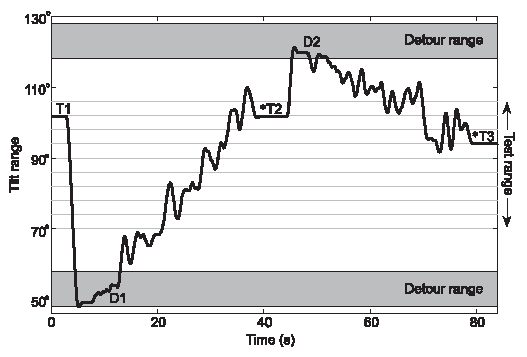
\includegraphics[width=0.5\textwidth]{src/paper1/figure2.pdf}
    
    \caption{Tilt paradigm in \SBT{90} task. T1, T2, T3, Test angles at which the subject was prompted with a beep signal (*) to indicate whether body orientation was CW or CCW from the instructed reference orientation (i.e., 90\mydegree in this example). D1, D2, Detour angles randomly drawn from detour range (30 - 40\mydegree CW and CCW from center of test range). Rotations from detour (D) to test (T) angle were performed in a noisy fashion (see \nameref{p1:sec:methods}, \nameref{p1:sec:methods_sbt}).}
    \label{p1:fig2}
\end{wrapfigure}

Each experimental run started in upright position with the room lights on. After the lights were turned off, subjects were first rotated at a constant angular velocity of 30\textdegree/s to a random detour angle, outside of the test angle range, where they remained for 3 s. The chair then moved to a randomly chosen position within the test range with a very slow and noisy profile, defined by the sum of a ramp of 0.4 - 2\textdegree/s and Gaussian white noise (bandwidth, 0 - 0.7 Hz; RMS amplitude, 3.4\textdegree). Ramp speed was chosen such that the trajectory between detour angle and test angle was reached in 30 s (Fig. \ref{p1:fig2}). These precautions were taken to enforce independent absolute tilt judgments and to deter reliance on sensed changes in tilt position that had occurred since the previous trial. Three seconds after arrival at the test angle, a beep signal prompted the subject to indicate whether body orientation was CW or CCW from the instructed reference orientation (0\mydegree in the \SBT{0} task, \textpm45\mydegree in the \SBT{\textpm45}, or \textpm90\mydegree in the \SBT{\textpm90} task), using a toggle switch. The subject was then rotated at a constant velocity to a new randomly drawn detour angle, and the above procedure was repeated. Each run, comprising seven test angles, lasted \textapprox5 min, after which the subject was rotated back to upright, and room lights were turned on. Between runs, there was a 60 s rest interval before the next run started. Each SBT task was tested in separate sessions of \textapprox45 min each, thus amounting to a total of 15 sessions per subject (i.e., \textapprox11 h of recording time).

\subsubsection{SVV}
 
The same subjects were also tested in a series of SVV experiments. Part of this dataset (four subjects) has been published previously as part of a larger dataset on visual verticality perception \cite{devrijer2009}. Data in the other three subjects were collected anew. Here we provide a brief summary of the paradigm. SVV was tested at nine roll-tilt angles, ranging from -120 to 120\mydegree at 30\mydegree intervals. A luminous line (angular subtend, 20\textdegree), polarized with a bright dot at one end, was mounted in front of the subject. The line's rotation axis coincided with the chair rotation axis. In each experimental run, the subject was rotated from upright to the chosen test angle at a constant angular velocity of 30\textdegree/s. After a 30 s waiting period that allowed canal effects to subside, a luminous line was briefly flashed (20 ms), and the subject indicated whether its orientation in space was CW or CCW from the perceived direction of gravity. The line orientation was selected randomly from a set of 11 line orientations. After all line orientations had been tested, the subject was rotated back to upright, and room lights were turned on. Positive and negative body-tilt angles were alternated regularly. As in the SBT experiment, we used the method of constant stimuli. The set of 11 line orientations was centered on a coarse estimate of the SVV threshold at each tilt angle. We used orientation intervals of 3\textdegree, except for upright, where intervals of 2\mydegree were taken. Each set of line orientations was tested in random order in 12 experimental runs, thus yielding a total of 132 responses for each psychometric curve. SVV data were collected in a total of five 45 min sessions per subject. 

\subsection{Data analysis}

CW tilt angles of the body and the luminous line were defined positive. We quantified performance, for each roll-tilt angle (5 in the SBT and 9 in the SVV) independently, by examining the proportion of CW responses as a function of body orientation (SBT) and the proportion of CCW responses as a function of line orientation with respect to the body (SVV). Psychometric data were quantified by fitting a cumulative Gaussian function (Fig. \ref{p1:fig3}): 

\begin{equation}
\label{p1:eqn1}
P(x) = \lambda + (1 - 2\lambda) \frac{1}{\sigma \sqrt{2\pi}} \int_{-\infty}^{x}{e^{-(y-\mu)^2 / 2\sigma^2}}dy,
\end{equation}
% Equation 1


in which $x$ represents body orientation in space (SBT experiment) or line orientation with respect to the body (SVV experiment). The mean of the Gaussian $\mu$ represents the subjective perception of the reference orientation in the SBT task, or the SVV compensation angle (the angle between the apparent visual vertical line and the body axis) in the SVV task. The width of the curve, $\sigma^2$, inversely related to precision, serves as a measure of the subject's variability in the SBT or SVV task. Parameter $\lambda$, representing the lapse rate, accounts for stimulus-independent errors caused by subject lapses or mistakes and was restricted to small values ($\lambda < 0.06$). Fits were performed using Matlab software (MathWorks) with the ``psignifit'' \cite{wichmann2001b} routine. 

\subsection{Sensory integration model}

To provide a theoretical framework that explains the observed responses, we designed a sensory integration model for visual verticality and body-tilt perception that assumes optimal processing of all potentially relevant sensory signals, including body, head, and neck sensors. The model links accuracy and variability in the two spatial tasks to the properties of the underlying sensors. For simplicity, the scheme is limited to SBT and SVV signal processing in darkness. 

In the scheme (Fig. \ref{p1:fig1}), we use the following conventions: physical variables are denoted by a capital with a subscript indicating the frame of reference. For example, $H_S$ represents the physical orientation of the head in space. Sensory signals and their reference-frame-transformed counterparts are denoted by a hat symbol (\textasciicircum), as in $\hat{H}_{S}$, which represents the orientation of the head in space as measured by the head-in-space sensors. The optimal estimate of a variable, obtained by integration of all available information, is indicated by a tilde (\textasciitilde), as in $\tilde{H}_S$, representing the final head-in-space estimate. 

It is assumed that all sensory signals are accurately calibrated (i.e., unbiased) but corrupted by independent Gaussian noise with a given variance ($\sigma^2$), with subscripts to indicate the sensory modality (e.g., $\sigma_{BS}^2$ represents noise variance in the body-in-space sensors). 

\subsubsection{SBT computation}
\label{p1:sec:sbt_computation}
 
To obtain an estimate of the orientation of the body in space, the brain can use ``direct'' sensory information from body sensors ($\hat{B}_S$), such as tactile receptors in the skin or so-called graviceptors in the trunk \cite{mittelstaedt1997, mittelstaedt1998, vaitl2002}. Alternatively, an ``indirect'' pathway, involving a reference frame transformation, can also provide a body-in-space estimate. For this purpose, sensory head-in-space information, provided by the otoliths, must be combined with information about head-on-body orientation, provided by proprioceptive signals from the neck ($\hat{B}_{SI} = \hat{H}_S - \hat{H}_B$). Because the sensors are contaminated by noise, the direct and indirect signals can be represented as Gaussian probability distributions with mean values of $\hat{B}_S$ and $\hat{H}_S - \hat{H}_B$, and variance levels of $\sigma_{BS}^2$ and $\sigma_{HS}^2 + \sigma_{HB}^2$, respectively. Theoretically, as shown in Figure \ref{p1:fig1}, the brain could also use prior information about body-in-space orientation in the computation of the body-in-space estimate. The effect of including a prior on the SBT (centered on upright) would be a systematic error of underestimation at larger tilt angles. However, neither previous findings \cite{mittelstaedt1983, mast1996, jarchow1999, vanbeuzekom2001} nor the present results (Figs. \ref{p1:fig3}, \ref{p1:fig4}), showed such systematic errors across subjects. In modeling terms, this indicates a uniform (uninformative) prior, which corresponds to a weight of 0. Accordingly, a statistically optimal estimate of body-in-space orientation ($\tilde{B}_S$) is then given by the peak of the Gaussian distribution that results from the multiplication of the two distributions representing the direct and indirect sensory pathways. It follows that

\begin{equation}
\label{p1:eqn2}
\tilde{B}_S = w_{BD} \cdot \hat{B}_S + w_{BI} \cdot (\hat{H}_S - \hat{H}_B),
\end{equation}

with

\begin{equation}
\label{p1:eqn3}
w_{BD} = \frac{1/\sigma^2_{BS}}{1/(\sigma^2_{HS} + \sigma^2_{HB}) + 1/\sigma^2_{BS}}
\end{equation}

and

\begin{equation}
\label{p1:eqn4}
w_{BI} = \frac{1/(\sigma^2_{HS} + \sigma^2_{HB})}{1/(\sigma^2_{HS} + \sigma^2_{HB}) + 1/\sigma^2_{BS}}
\end{equation}

in which $w_{BD}$ and $w_{BI}$ (Fig. \ref{p1:fig1}) represent the respective weights of the direct and indirect pathways, which add up to 1 \cite{landy1995,jacobs1999,ernst2002,bays2007}. Note that the weight of each pathway depends on its reciprocal noise variance (also known as precision), so that precise signals have a stronger influence on the final estimate than noisy signals. Furthermore, because both sensory pathways are supposed to carry unbiased signals, the mean estimate of body in space in multiple trials, $\mu(\tilde{B}_S)$, will also be accurate. 

It can further be shown that the variance in $\tilde{B}_S$ in multiple trials, denoted as $\sigma^2(\tilde{B}_S)$, equals 

\begin{equation}
\label{p1:eqn5}
\sigma^2(\tilde{B}_S) = \frac{
\sigma^2_{BS} \cdot (\sigma^2_{HS} + \sigma^2_{HB})
}{
\sigma^2_{BS} + (\sigma^2_{HS} + \sigma^2_{HB})
}
\end{equation}

which implies that the final estimate has a lower variance than the signal provided by either the direct or the indirect pathway \cite{ernst2002,ernst2004}. Because we assume that sensory signals are accurate and that there is no prior information about body in space, the model predicts that there are no systematic errors in the SBT, so that $\mu(\tilde{B}_S) = B_S$. The variance in the SBT task is represented by $\sigma^2(\tilde{B}_S)$. 

\subsubsection{SVV computation}

The scheme applies a similar sensory signal processing strategy to estimate the orientation of head in space, $\tilde{H}_S$, used in the SVV. A direct estimate of head-in-space orientation is provided by the head-in-space sensors ($\hat{H}_S$), and an indirect estimate is obtained by a reference frame transformation of the body-in-space signal ($\hat{B}_S$) by adding the head-on-body estimate ($\hat{H}_B$), provided by the neck sensors ($\hat{H}_{SI} = \hat{B}_S + \hat{H}_B$). Again, direct and indirect pathway signals are represented by two Gaussian probability distributions, with mean values of $\hat{H}_S$ and $\hat{B}_S + \hat{H}_B$, respectively, and corresponding variances of $\sigma^2_{HS}$ and $\sigma^2_{BS} + \sigma^2_{HB}$. In the computation of the head-in-space estimate, to account for systematic errors \cite{macneilage2007, devrijer2008}, it is further assumed that the brain uses prior knowledge about head-in-space orientation, which entails that small head-tilt angles are considered more probable than large tilts. Mathematically, the prior is represented by a Gaussian distribution that is centered at 0\mydegree head tilt ($H_{SP} = 0^\circ$) with a variance of $\sigma^2_{HSP}$. Note that, in our scheme, the head-in-space prior, which contributes to the SVV computations, does not affect the body-in-space estimate. Integration of the direct and indirect sensory pathways and prior knowledge is performed by multiplication of the three Gaussian distributions. The peak of the resulting posterior distribution represents the optimal estimate of head-in-space orientation ($\tilde{H}_S$), which is given by the following: 

% Equation 6
\begin{equation}
\label{p1:eqn6}
\tilde{H}_S = w_{HD} \cdot \hat{H}_S + w_{HI} \cdot (\hat{B}_S + \hat{H}_B) + w_{HP} \cdot H_{SP}
\end{equation}

with

% Equation 7/8
\begin{equation}
\label{p1:eqn7}
w_{HD} = \frac{1 / \sigma^2_{HS}}{1 / (\sigma^2_{BS} + \sigma^2_{HB}) + 1/\sigma^2_{HS} + 1/\sigma^2_{HSP}},
\end{equation}

\begin{equation}
\label{p1:eqn8}
w_{HI} = \frac{1 / (\sigma^2_{BS} + 1/\sigma^2_{HB})}{1 / (\sigma^2_{BS} + \sigma^2_{HB}) + 1/\sigma^2_{HS} + 1/\sigma^2_{HSP}}
\end{equation}
% Check eqn. 8 the 2nd 1/ might be a mistake

and

\begin{equation}
\label{p1:eqn9}
w_{HP} = \frac{1 / \sigma^2_{HSP}}{1 / (\sigma^2_{BS} + \sigma^2_{HB}) + 1/\sigma^2_{HS} + 1/\sigma^2_{HSP}}
\end{equation}
% Equation 9

In this equation, $w_{HD}$, $w_{HI}$, and $w_{HP}$ (which add up to one) represent the weights of the direct and indirect pathways and the prior, respectively, which are proportional to the relative precision of the sensory signals and the width of the prior. Equation \ref{p1:eqn6} would result in an accurate estimate of $\tilde{H}_S$, if all three pathways were accurate by themselves. However, because the prior is centered on zero ($H_{SP} = 0\degree$), it introduces more and more bias toward upright, as head tilt increases further. Thus, optimization in terms of variance has a downside by causing underestimation of the actual head tilt. The amount of underestimation depends on the width of the prior and the reliability of the sensory inputs.

The variance in the head-in-space estimates, measured across many trials, $\sigma^2(\tilde{H}_S)$, can be derived directly from Equation \ref{p1:eqn6} by applying the rules of error propagation (see \nameref{p1:sec:appendix} for complete derivation). From these calculations, it follows that 

% Equation 10
\begin{equation}
\label{p1:eqn10}
\sigma^2(\tilde{H}_{S}) = w^2_{HD} \cdot \sigma^2_{HS} + w^2_{HI} \cdot (\sigma^2_{BS} + \sigma^2_{HB}),
\end{equation}

in which the variance contributions of the direct and indirect pathways are represented by their squared weights. Although it does not appear explicitly in Equation \ref{p1:eqn10}, it is important to notice that the prior has a noise-reducing effect by downscaling the sensory-related weighting terms ($w_{HD}$ and $w_{HI}$). The narrower the prior, the larger its relative weight ($w_{HP}$) and the smaller the sensory weights, because $w_{HD} + w_{HI} + w_{HP} = 1$. Thus, the effect of the head-in-space prior is twofold: it reduces the variance, but as noticed above, this occurs at the cost of a bias in the final estimate of head-in-space orientation, which becomes pronounced at large tilts (see \nameref{p1:sec:appendix} for further details). 

Previously, we have shown that to account for the typical nonlinear increase of the systematic SVV errors with tilt, the variability of the head-tilt signal in the model must increase with tilt angle \cite{devrijer2008,devrijer2009}. In line with this conclusion, decreasing effectiveness of the otoliths with increasing tilt has been suggested by various other reports \cite{schone1968,tarnutzer2009,tarnutzer2010} and may reflect the geometry of otolith organs, the nonuniform distribution of otolith afferents in the roll-plane and nonlinear firing rates \cite{tarnutzer2010}. This feature was incorporated by allowing the noise in the sensory head-tilt signal, $\sigma_{HS}$, to increase rectilinearly with tilt angle: 

% Equation 11
\begin{equation}
\label{p1:eqn11}
\sigma_{HS} = a_{HS} |H_S| + b_{HS}
\end{equation}

in which $a_{HS}$ reflects the proportional increase of noise with tilt angle and $b_{HS}$ represents the noise at $H_{S} = 0\degree$. Note that, in the data fits, parameter $a_{HS}$ was allowed to be zero, so that the present model did not force $\sigma_{HS}$ to depend on head tilt. 

To compute the SVV, the brain not only requires an estimate of head orientation in space ($\tilde{H}_S$), but also needs estimates of eye-in-head orientation ($\tilde{E}_H$) and retinal line orientation ($\tilde{L}_E$). Together, these signals determine the orientation of a visual line in space ($\tilde{L}_S$) according to $\tilde{L}_S = \tilde{H}_S + \tilde{E}_H + \tilde{L}_E$. The systematic error in the SVV experiment (${\Delta}SVV$) corresponds to the error in $\tilde{L}_S$ and is thus given by ${\Delta}SVV = {\Delta}H_S + {\Delta}E_H + {\Delta}L_E$, in which $\Delta$ denotes the bias in each estimate. For simplicity, we assumed that the visual signal representing retinal line orientation is accurate, so that ${\Delta}L_E = 0\degree$. As explained in a previous study \cite{devrijer2009}, underestimation of eye torsion causes errors in the eye-in-head estimate (${\Delta}E_H$), which can be represented by ${\Delta}E_H = -A_{OCR} \cdot \sin(\hat{H}_S$, where parameter $A_{OCR}$ denotes uncompensated ocular counterroll. Finally, the error in the head-in-space estimate is obtained by subtracting $\tilde{H}_S$ (see Eq. \ref{p1:eqn6}) from the actual head tilt $H_S$, which ultimately leads to the following relation for the mean SVV error, $\mu({\Delta}SVV)$, in multiple trials: 

% Equation 12
\begin{equation}
\label{p1:eqn12}
\mu({\Delta}SVV) = (1 - w_{HD} - w_{HI}) \cdot H_S - A_{OCR} \cdot \sin(H_S)
\end{equation}

In Equation \ref{p1:eqn12}, the influence of the prior works through the weight factors $w_{HD}$ and $w_{HI}$. Because these weights do not add up to 1 (see above, $w_{HD} + w_{HI} = 1 - w_{HP} < 1$), the result is a systematic error in the head-in-space estimate, which becomes more pronounced at large tilt. The noise level in the eye-in-head and line-on-eye estimates is probably relatively small compared with the noise in the head-in-space estimate considering results from Vandenbussche et al. \citeyear{vandenbussche1986}, who reported just-noticeable difference levels for orientation discrimination of \textless1\textdegree. Given this low value, SVV variance is determined mainly by the variance in the latter estimate, so that $\sigma^2({\Delta}SVV) \sim \sigma^2(\tilde{H}_S)$.

\subsection{Model fitting}

The model contains seven fit parameters ($a_{HS}$, $b_{HS}$, $\sigma_{HSP}$, $\sigma_{BS}$, $\sigma_{HB}$, $A_{OCR}$, and $\lambda$) that were fitted to all data (SBT and SVV) simultaneously for each subject. As stated earlier, parameters $a_{HS}$ and $b_{HS}$ represent the increase and offset of sensory noise in the head-in-space estimate, respectively. The parameter $\sigma_{HSP}$ denotes the width of the prior distribution, reflecting a priori knowledge about head-in-space. Noise levels in the body and neck sensors are represented by parameters $\sigma_{BS}$ and $\sigma_{HB}$. Finally, the amplitude of uncompensated ocular counterroll is denoted by $A_{OCR}$. In addition to these six parameters related to sensory processing, there is a seventh parameter to account for lapses ($\lambda$). 

In addition to these ``parameters of interest'', the data were preprocessed before model fitting by applying mean correction \cite{mcguire2009}. Mean correction was performed to remove systematic errors in the SBT and the asymmetries in the SVV between CW and CCW tilt angles. Because the model is inherently left-right symmetric, it would try to account for differences in SVV bias between equal but opposite tilt angles by falsely increasing the variance. Likewise, because the model assumes that there is no bias in the SBT, it would try to explain any slight deviation from zero by excessively increasing the variance. The asymmetry in the SVV, if any, and a nonzero SBT bias, if any, are captured by fixed parameters of noninterest (n = 9) in the model fits. Thus, for the SBT data, one bias correction term was needed for each tilt angle (yielding five parameters of noninterest), and for the SVV data, one correction parameter was needed for each pair of equal but opposite tilt angles (yielding four parameters of noninterest). We emphasize that the nine parameters of noninterest are not free-fit parameters because they are not optimized by the model. So, although technically our number of free parameters amounts to a total of 16, only seven were determined by fitting the model. 

In total, the seven free parameters of the model had to account for 149 data points, spread across various tilt angles, with each data point reflecting a proportion of CW responses based on either 14 (for the SBT) or 11 (for the SVV) experimental forced-choice CW/CCW responses. We fitted the model by maximizing the likelihood of the data [maximum likelihood estimation (MLE)], in relation to the set of six model parameters ($a_{HS}$, $b_{HS}$, $\sigma_{HSP}$, $\sigma_{BS}$, $\sigma_{HB}$, and $A_{OCR}$) and lapse rate ($\lambda$). Optimal parameter values were obtained by minimizing the negative likelihood function using the Matlab function ``fmincon'' \cite{devrijer2008, mcguire2009}. Simulations confirmed that the inverse modeling approach was not sensitive to overfitting. SDs of the best-fit parameters were obtained by performing 1999 bootstrap runs. For each run, we constructed 149 data points (reflecting the size of the dataset), each of which was obtained by random sampling with replacement from the original dataset. The model was fit to this new dataset. The distribution of model parameters across all runs was used to derive the 68.2\% confidence interval of each parameter. 

We emphasize that the model fit provided an estimate of the proprioceptive variance of the neck ($\sigma_{HB}$), even though the head-on-body signal was not directly manipulated during the experiment. Nevertheless, this signal, as sensed by the neck proprioceptors, is essential to implement the reference frame transformation from the body-in-space to the head-in-space signal, and vice versa. Because the neck signal is noisy, these reference frame transformations induce neck-related noise in the original $B_S$ and $H_S$ signals, even when the head and body are aligned. Because the SBT and SVV tasks require different reference frame transformations, they depend differently on the noise properties of the three sensory systems (body and neck sensors and otoliths). By solving the inverse problem, the noise properties of the three sensory systems, as well as the other fit parameters, can be determined. Finally, we note that the inverse problem can only be solved using both tasks at multiple tilt angles; just using a single task (SVV or SBT, not both) would have made this problem intractable. 

\subsection{Model evaluation}

To assess the importance of cross-modal sensory integration, we also fitted our model without the indirect, cross-modal pathways by setting the head-on-body noise to infinity, which effectively eliminates the indirect pathways and removes one degree of freedom. To compare the maximum-likelihood estimates from the full and the reduced model, we used a log-likelihood ratio test. The test statistic is two times the difference between the negative log-likelihoods of the data, given the reduced and the full model. A $\chi^2$ test with one free parameter (the difference in degrees of freedom between the two models) is used to calculate the $p$ value \cite{dobson2001}.

Furthermore, we evaluated our mechanistic model in comparison with a pure descriptive model of the same dataset based on separate psychometric accounts, each with three free parameters, at the five SBT and nine SVV angles. We used the Bayesian information criterion (BIC) for model comparison. BIC provides a measure of the adequacy of the model fit and corrects for the number of parameters. The BIC is defined as $BIC = -2 \log(L) + k \cdot \log(n)$, in which $L$ is the total likelihood of the data given the model, $k$ the number of free parameters, and $n$ the number of data points to be explained. The number of free parameters is 42 [14 psychometric curves $\times$ 3 parameters ($\mu$, $\sigma$, and $\lambda$)] for the psychometric curves, whereas for the mechanistic Bayesian model, the number of free parameters is seven. A more appropriate model is characterized by a lower BIC value. 

%%%% ^^^ Fixme x should be cross

\subsection{Model validation: independent test of neck noise}

The SBT and SVV measurements to test the model proposed in Figure 1 have yielded solutions for the noise properties of the involved sensor systems. To validate the model structure and the noise predictions that were obtained, we also devised an experiment that independently measured the noise in the neck sensors (head-on-body sensors), in a psychometric fashion. In this experiment, subjects were lying on a bed, in supine position, with their head fixed on a rotating platform. The platform was constructed such that it could passively rotate the head relative to the body, in the roll plane, while accounting for the shifting rotation axis in the neck vertebrae. The rotation of the platform was computer controlled, keeping the speed below $0.2{\degree}/s$, which is far below detection threshold of the canals ($>0.5{\degree}/s$) (Benson et al., 1989). In the supine condition, there is no gravity modulation of the otolith signal, so we excluded the contribution of the vestibular system in detecting head-on-body orientation and were only probing the role of the neck afferents. We applied the method of constant stimuli, using a set of 11 head angles relative to body midline. Test angles ranged from $-6\degree$ to $6\degree$. 

In complete darkness, subjects were first rotated at a constant angular velocity of =15∞/s to a random detour angle similar to the idea shown in Figure 2. The head then moved to a randomly chosen position within the test range with a very slow speed ($<0.2{\degree}/s$) such that the test angle was reached within 20s. Meanwhile, auditory white noise was presented to the subjects through earphones to mask any auditory cues generated by the moving platform. After arrival at the test angle, the auditory noise was interrupted, signaling the subject to indicate whether head-on-body orientation was CW or CCW relative to the body midline, using a toggle switch. The subject was then rotated at a constant velocity to a new randomly chosen detour angle, and the above procedure was repeated. Each test angle was repeated 10 times, yielding a total number of 110 responses in each subject. Psychometric data were quantified by fitting a cumulative Gaussian function (see above, Eq. 1). The width of the curve, $\sigma^2$, inversely related to precision, serves as an independent measure of the subject's variability of the head-on-body estimate and was compared with the model prediction. 

\subsection{Model simulation of patient data}

Based on the average parameter values of the model established in normal, healthy subjects, the model was also used to make predictions about SVV and SBT performance in two patient groups: bilateral vestibular patients and patients with somatosensory loss. The model simulated SVV and SBT in these patient groups by raising the variance values of the lost signals to infinity. 